\documentclass{classes/fiboreport}

\begin{document}

\Modifydate{25/05/2018}
\subject{ENE495 Internet of Things}
\title{Automotive Minions}
\subtitle{รถจัดเก็บสินค้าอัตโนมัติ}
\academicyear{2560}
\coverimage{cover.jpg}
\covertext{
	\begin{tabular}{ l l }
		{นายจุฬภัทร จิรชัย} & {57340500013} \\  
		{นายเจตนันท์ หอมจันทนากุล} & {57340500015} \\
		{นายวุฒิภัทร โชคอนันตทรัพย์} & {57340500067} \\ 
		{นายศิรวัชร ศกศวัตเมฆิทร์} & {57340500071} 
	\end{tabular}
}
\pagecolor{tudelft-orange}
\maketitle

% % ************************** Thesis Abstract **********************************
\begin{abstract}
	สำหรับเขียนบทคัดย่อ
\end{abstract}
\tableofcontents
\listoffigures
% % ***************************** Thesis Symbols ********************************
\begin{symbols}
    \noindent
    \begin{tabular*}{\textwidth}{@{}p{0.18\textwidth}p{0.8\textwidth}@{}}
        {$\theta$} & {เซต้า} \\
        {$d$} & {distance} \\
        {kg} & {Kilogram} \\
        {m$^{2}$} & {Square Metre} \\
    \end{tabular*}
\end{symbols}
% % ************************** Thesis Abbreviations **************************
\begin{abbreviations}
    \noindent
    \begin{tabular*}{\textwidth}{@{}p{0.18\textwidth}p{0.8\textwidth}@{}}
        {CW} & {Clockwise} \\
        {CCW} & {Counterclockwise} \\
        {UTHAI} & {Universal Template for Humanoid Algorithm Interface} \\
        {ROS} & {Robot Operating System} \\
        {IMU} & {Inertial Measurement Unit} \\
        {DoF} & {Degree of Freedom} \\
        {CoM} & {Center of Mass} \\
        {ZMP} & {Zero Moment Point} \\
        {PLA} & {Polylactic acid} \\
        {ABS} & {Acrylonitrile butadiene styrene} \\
        {KMUTT} & {King Mongkut's University of Technology Thonburi} \\
        {Liews} & {วุฒิภัทร โชคอนันตทรัพย์} \\
        {$\theta$} & {เซต้า}
    \end{tabular*}
\end{abbreviations}


\chapter{บทนำ}
\section{ที่มาและความสำคัญ}
ในปัจจุบันการเคลื่อนย้ายสินค้าต่างๆภายในโรงงานยังใช้แรงงานมนุษย์อยู่ โดยวิธีการทั่วไปที่โรงงานนิยมใช้คือ
การใช้รถเข็นลำเลียงเพื่อเคลื่อนย้ายสินค้า ซึ่งผู้ที่ใช้รถเข็นจะต้องมีประสบการณ์ในการใช้ และต้องมีการระวังอยู่ตลอดการใช้งานรถเข็น
แต่เนื่องจากการทำงานของมนุษย์มีความเสี่ยงที่จะทำให้เกิดความผิดพลาดได้สูงจากปัจจัยหลายอย่าง เช่น
การพักผ่อนไม่เพียงพอ สภาพร่างกายไม่พร้อม สถาพจิตใจที่ไม่พร้อม อารมณ์ต่างๆ ซึ่งความผิดพลาดจะนำมาซึ่งความเสียหายต่อโรงงานได้
ดังนั้นการพัฒนารถขับเคลื่อนอัตโนมัติ AGV (Automated Guided Vehicle) ซึ่งเป็นเครื่องจักรชนิดหนึ่งที่ใช้คอมพิวเตอร์ในการควบคุม
มีความสามารถในการเดินทางตามเส้นทางที่กำหนดไว้ การนำรถขับเคลื่อนอัตโนมัติมาเพื่อทดแทนการทำงานของมนุษย์ในส่วนนี้จึงเป็นสิ่งสำคัญ
โดยนอกจากจะตัดปัญหาในส่วนการทำงานที่ผิดพลาดแล้ว ยังช่วยให้โรงงานมีประสิทธิภาพในการบริหารจัดการคลังสินค้ามากขึ้น
ด้วยแนวคิดดังกล่าวจึงทำให้เกิดหัวข้อโครงงานนี้ขึ้นมา

\section{วัตถุประสงค์}
วัตถุประสงค์ในการทำโครงงานนี้ขึ้นมาก็เพื่อที่จะได้พัฒนาระบบการเคลื่อนย้ายลำเลียงสินค้าอัตโนมัติภายในคลังสินค้า
พัฒนาระบบการขับเคลื่อนของหุ่นยนต์สองล้อสำหรับใช้ในการขนย้ายสินค้า และได้ประยุกต์ใช้ IoT (Internet of Things)
กับระบบจัดเก็บคลังสินค้าภายในโรงงานอุตสาหกรรม

\section{ขอบเขตของโครงงาน}
\begin{enumerate}[label=\thesection.\arabic*, leftmargin=1.5cm]
	\setlength\itemsep{-0.25em}
	\item ออกแบบและพัฒนาระบบการเคลื่อนย้ายสินค้าภายในคลังสินค้าอัตโนมัติ
	\item จำลองรถขับเคลื่อนอัตโนมัติโดยใช้หุ่นยนต์สองล้อ (Differential Drive Robot)
	\item ออกแบบและพัฒนาให้หุ่นยนต์เคลื่อนที่ไปยังตำแหน่งที่กำหนดได้
	\item ออกแบบและพัฒนาระบบ Cyber-Physical System (CPS) ให้กับการทำงานของ AGV
\end{enumerate}


% เป็นโครงงานที่พัฒนาระบบการรับ-ส่ง เคลื่อนย้ายสินค้าเพื่อจัดเก็บในคลังสินค้าแบบอัตโนมัติ โดยใช้ AGV
% ซึ่งจะจำลองให้อยู่ในรูปแบบของหุ่นยนต์ขับเคลื่อนสองล้อ
% โดยหุ่นยนตส์ ามารถยกสินคา้ แลว้เดินไปวางตามจุดจดัเก็บที่กา หนดโดยใชเ้ส้นในการนา ทาง ซ่ึงจะแยก
% สินค้าโดยใช้ Image Processing, QR Code หรือ Bar Code แลว้จะทา การส่งขอ้มูลไปบน Cloud เพื่อ
% ประมวลผลในการแยกสินคา้และกา หนดจุดจดัเก็บสินคา้และเพื่อแสดงใหผ้ใู้ชส้ ามารถรับรู้วา่ หุ่นยนต์
% กา ลงัขนสินคา้ชนิดใด จากน้นัจะทา การส่งขอ้มูลกลบัไปยงัหุ่นยนตเ์พื่อใหห้ ุ่นยนตจ์ดัเก็บสินคา้ตามจุด
% จดัเก็บที่กา หนดได้ และเมื่อส่งสินคา้เสร็จแลว้ก็จะส่งสถานการณ์ทา งานกลบั มายงั Cloud เพื่อจดัเก็บ
% ข้อมูล ซ่ึงหุ่นยนตจ์ะส่งขอ้มูลที่เกี่ยวขอ้งกบั ตวัหุ่นยนตเ์องข้ึนไปบนระบบดว้ย ซ่ึงขอ้ มูลของตวัหุ่นยนต์
% จะประกอบไปด้วย Workload และ Voltage
% ส่วนของฝั่ง Cloud Server น้นั จะใชเ้ป็นของ Azure (Microsoft) โดยจะมีเครื่องมือที่ใชท้ ้งัหมด 5
% อยา่ งดว้ยกนัคือ Azure IoT Hub,Stream Analytics, Power Bi, Machine Learning และ Azure Storage โดย
% ข้นั ตอนในการทา งานคือ ทา การเก็บขอ้มูลจากเซนเซอร์ต่าง ๆ ที่เกี่ยวขอ้งกบั หุ่นยนต์ส่งผา่ นมาให้Azure
% IoT Hub เพื่อทา การนา ขอ้ มูลไปใชใ้นส่วนต่าง ๆ ของ Microsoft’s Frameworkเช่น การทา Data Analytics
% ด้วย Machine Learning การท า Data Visualizationด้วยPower BI เป็ นต้น โดยหลงัจากส่งมาที่Azure IoT
% Hub จะส่งขอ้มูลต่อไปยงั Stream Analytics เพื่อ น าไปแสดงผลแบบ Real Time บน Power Bi (Web
% Applicationfor Data Visualization) โดยนอกจากการแสดงผลแล้ว จะน าข้อมูลที่ได้ไปท า Data Analytics
% โดยใช้ Machine Learning แลว้จะทา การเก็บขอ้มูลไวท้ี่ Azure Storage เพื่อเอาไว้ท าการวิเคราะห์และดู
% ข้อมูลย้อนหลัง

\chapter{ออกแบบระบบ}
\section{คำอธิบายโครงงาน}
เป็นโครงงานที่พัฒนาระบบการรับ-ส่งสินค้าเพื่อจัดเก็บใน Ware-House อัตโนมัติ โดยใช้ AGV
ซึ่งจะอยู่ในรูปแบบของหุ่นยนต์ขับเคลื่อนสองล้อ โดยหุ่นยนต์สามารถยกสินค้า
แล้วเดินไปวางตามจุดจัดเก็บที่กำหนดโดยใช้ Lidar ในการสร้างแผนที่เพื่อการนำทาง
และจะมีการส่งข้อมูลไปบน Cloud เพื่อแสดงผลให้ผู้ใช้สามารถรับรู้ถึงสถานะของหุ่นยนต์
จากนั้นจะทำการส่งข้อมูลกลับไปยังหุ่นยนต์เพื่อให้หุ่นยนต์จัดเก็บสินค้าตามจุดจัดเก็บที่กำหนดได้
และเมื่อส่งสินค้าเสร็จแล้วก็จะส่งสถานะการทำงานกลับมายัง Cloud เพื่อจัดเก็บข้อมูล
ซึ่งหุ่นยนต์จะส่งข้อมูลที่เกี่ยวข้องกับตัวหุ่นยนต์เองขึ้นไปบนระบบเพื่อนำไปประมวลผลและพัฒนาการทำงาน
โดยข้อมูลของตัวหุ่นยนต์จะประกอบไปด้วย น้ำหนักที่หุ่นยนต์แบกรับ แรงดันไฟฟ้าที่ใช้
กระแสไฟฟ้าที่ใช้ ระยะเวลาที่ใช้ในการทำงาน จุดเริ่มต้น จุดสิ้นสุด วันและเวลาที่ปฏิบัติงาน

\section{องค์ประกอบโดยรวมของระบบ}
\begin{figure}[!ht]
	\centering
	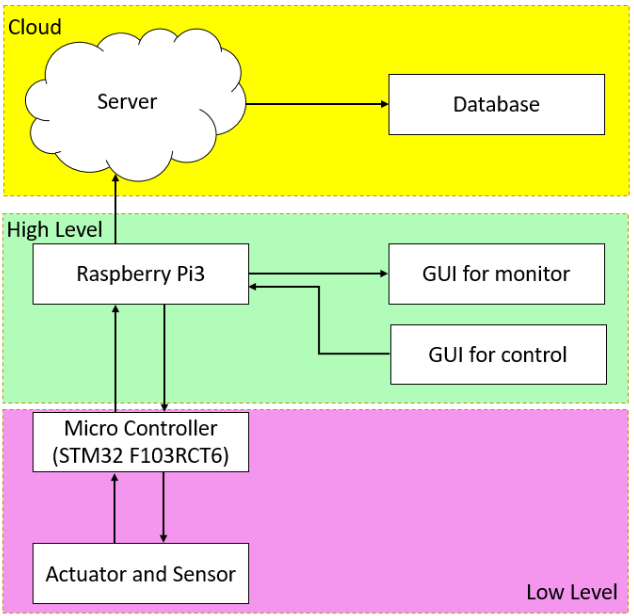
\includegraphics[width=0.8\textwidth]{images/system_overview.png}
	\caption{องค์ประกอบโดยรวมของระบบ}
	\label{fig:system_overview}
\end{figure}
\clearpage
ระบบสามารถแบ่งออกได้เป็น 3 องค์ประกอบใหญ่ด้วยกันคือ Cloud, High level และ Low level ดังรูปที่ \ref{fig:system_overview}
ซึ่งในแต่ละส่วนจะมีหน้าที่แตกต่างกันไปดังนี้

\subsection{Cloud}
เป็นส่วนประกอบที่นำมาใช้ในการจัดเก็บข้อมูลเพื่อให้สามารถนำผลลัพธ์ไปวิเคราะห์ประสิทธิภาพการทำงาน
หรือพฤติกรรมของระบบได้ มีองค์ประกอบทั้งหมด 2 ส่วนด้วยกันคือ Server และ Database โดย Server 
เปรียบเสมือนตัวกลางที่ใช้ในการรับส่งข้อมูลระหว่างอุปกรณ์และ Database ซึ่ง Database 
เป็นฐานข้อมูลที่ถูกใช้ในการเก็บข้อมูลเกี่ยวกับสถานะและประวัติการทำงานของหุ่นยนต์

\subsection{High Level}
เป็นส่วนที่ใช้ในการประมวลผลหลักเพื่อสั่งการและแสดงผลการทำงานต่างๆ โดยจะมี Raspberry Pi3
เป็นคอนโทรลเลอร์ที่ใช้ในการจัดการข้อมูลและประมวลผลรวมไปถึงการแสดงผลในรูปแบบต่างๆ
ซึ่งจะมี GUI for monitor ในการแสดงผลจากเซนเซอร์และอุปกรณ์ต่าง ๆ และมี GUI for control
ที่เป็นอุปกรณ์ที่ให้ผู้ใช้ได้ทำงานสั่งการระบบเพื่อให้หุ่นยนต์มีการทำงานตามคำสั่ง

\subsection{Low Level}
เป็นส่วนที่รับคำสั่งต่างๆ จาก High Level แล้วนำไปสั่งการกลไกและอุปกรณ์ต่างๆ
ให้มีการทำงานเป็นไปตามที่กำหนดไว้ และทำการอ่านค่าจากเซนเซอร์และอุปกรณ์ต่างๆ
เพื่อส่งข้อมูลกลับไปยัง High Level ได้ทำการประมวลผล แสดงผล และทำหน้าที่ในการตัดสินใจ
เพื่อสั่งงานให้หุ่นยนต์มีการทำงานอย่างมีระบบ





\chapter{พัฒนาระบบ}

\section{Hardware}
ฮาดแวร์พื้นฐานของหุ่นยนต์ขับเคลื่อน 2 ล้อตัวนี้จะประกอบไปด้วยฮาดแวร์ดังต่อไปนี้มอเตอร์
ไมโครคอนโทรลเลอร์  เซ็นเซอร์วัดแรง เซ็นเซอร์วัดแสงรอบทิศทางในแนวสองมิติ
และคอมพิวเตอร์ขนาดเล็ก โดยอุปกรณ์ทั้งหมดนี้จะมีการเชื่อมตัวกัน ดังรูปที่ \ref{fig:hardware}
\begin{figure}[!ht]
	\centering
	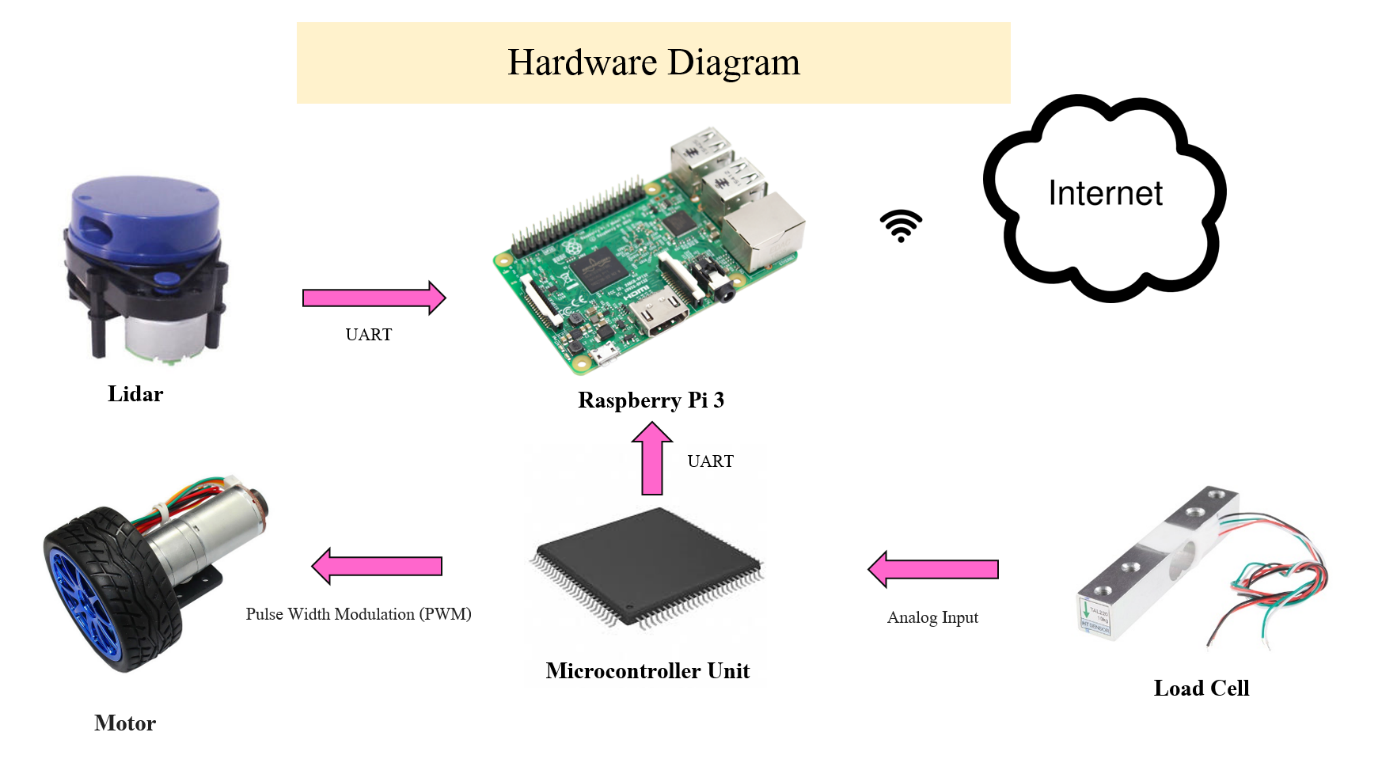
\includegraphics[width=0.9\textwidth]{images/hardware.png}
	\caption{ส่วนประกอบของหุ่นยนต์}
	\label{fig:hardware}
\end{figure}
ซึ่งรูปแบบในการเชื่อมต่อก็จะภายในฮาดแวร์กันเองก็จะมีที่ใช้ทั้งหมดหลักๆสามชนิดคือ 
1.PWM 2.UART 3.ADC
ส่วนการเชื่อมต่อจากฮาดแวร์ขึ้นไปบนซอฟแวร์นั้นจะผ่านทางสัญญาณไร้สาย
โครงสร้างของหุ่นยนต์เคลื่อนที่ 2 ล้อ ล้อและมอเตอร์จะถูกติดตั้งในลักษณะที่เรียกว่า
Differential drive เพราะว่าการติดตั้งแบบนี้จะมีข้อดี คือ การเลี้ยว หรือการหมุน
สามารถทำได้โดยตำแหน่งของหุ่นยนต์ยังอยู่ที่ดีเดิม ซึ่งเหมาะแก่การนำมาเป็นหุ่นยนต์ในการขนส่งสินค้าที่มีพื้นที่จำกัดได้
\begin{figure}[!ht]
	\centering
	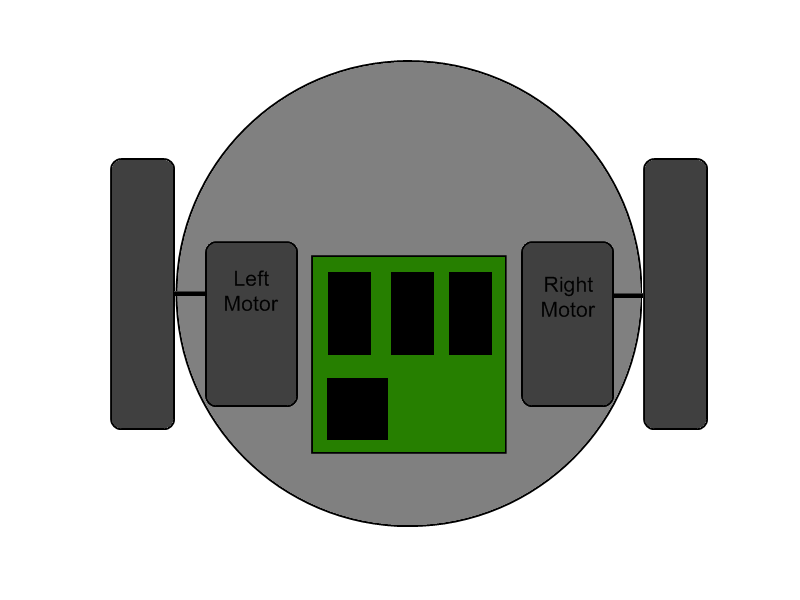
\includegraphics[width=0.5\textwidth]{images/robot.png}
	\caption{ลักษณะของหุ่นยนต์สองล้อ}
	\label{fig:robot}
\end{figure}

\clearpage
\section{Server and Database}
เป็นส่วนที่ใช้ในการเก็บข้อมูลต่างๆของหุ่นยนต์ทั้งหมด โดยหุ่นยนต์ทุกตัวจะเชื่อมต่อผ่าน Server เดียวกัน
ซึ่ง Server จะถูกสร้างขึ้นบน Microsoft Azure และหุ่นยนต์ทุกตัวมีการใช้ Database ร่วมกัน
แต่มีการใช้ตารางในการเก็บข้อมูลที่แตกต่างกัน โดยในแต่ละตารางจะมีทั้งหมด 10 หัวข้อ
ประกอบไปด้วย วันที่ทำงาน เวลาที่ทำงาน แรงดันไฟฟ้า กระแสไฟฟ้า น้ำหนักที่แบกรับ
ระยะทางที่ใช้ เวลาที่ใช้ จุดเริ่มต้น ปลายทาง และ อุณหภูมิ ณ ช่วงเวลานั้นๆ ซึ่งจะมีชนิดของตัวแปรดังนี้
\begin{figure}[!ht]
	\centering
	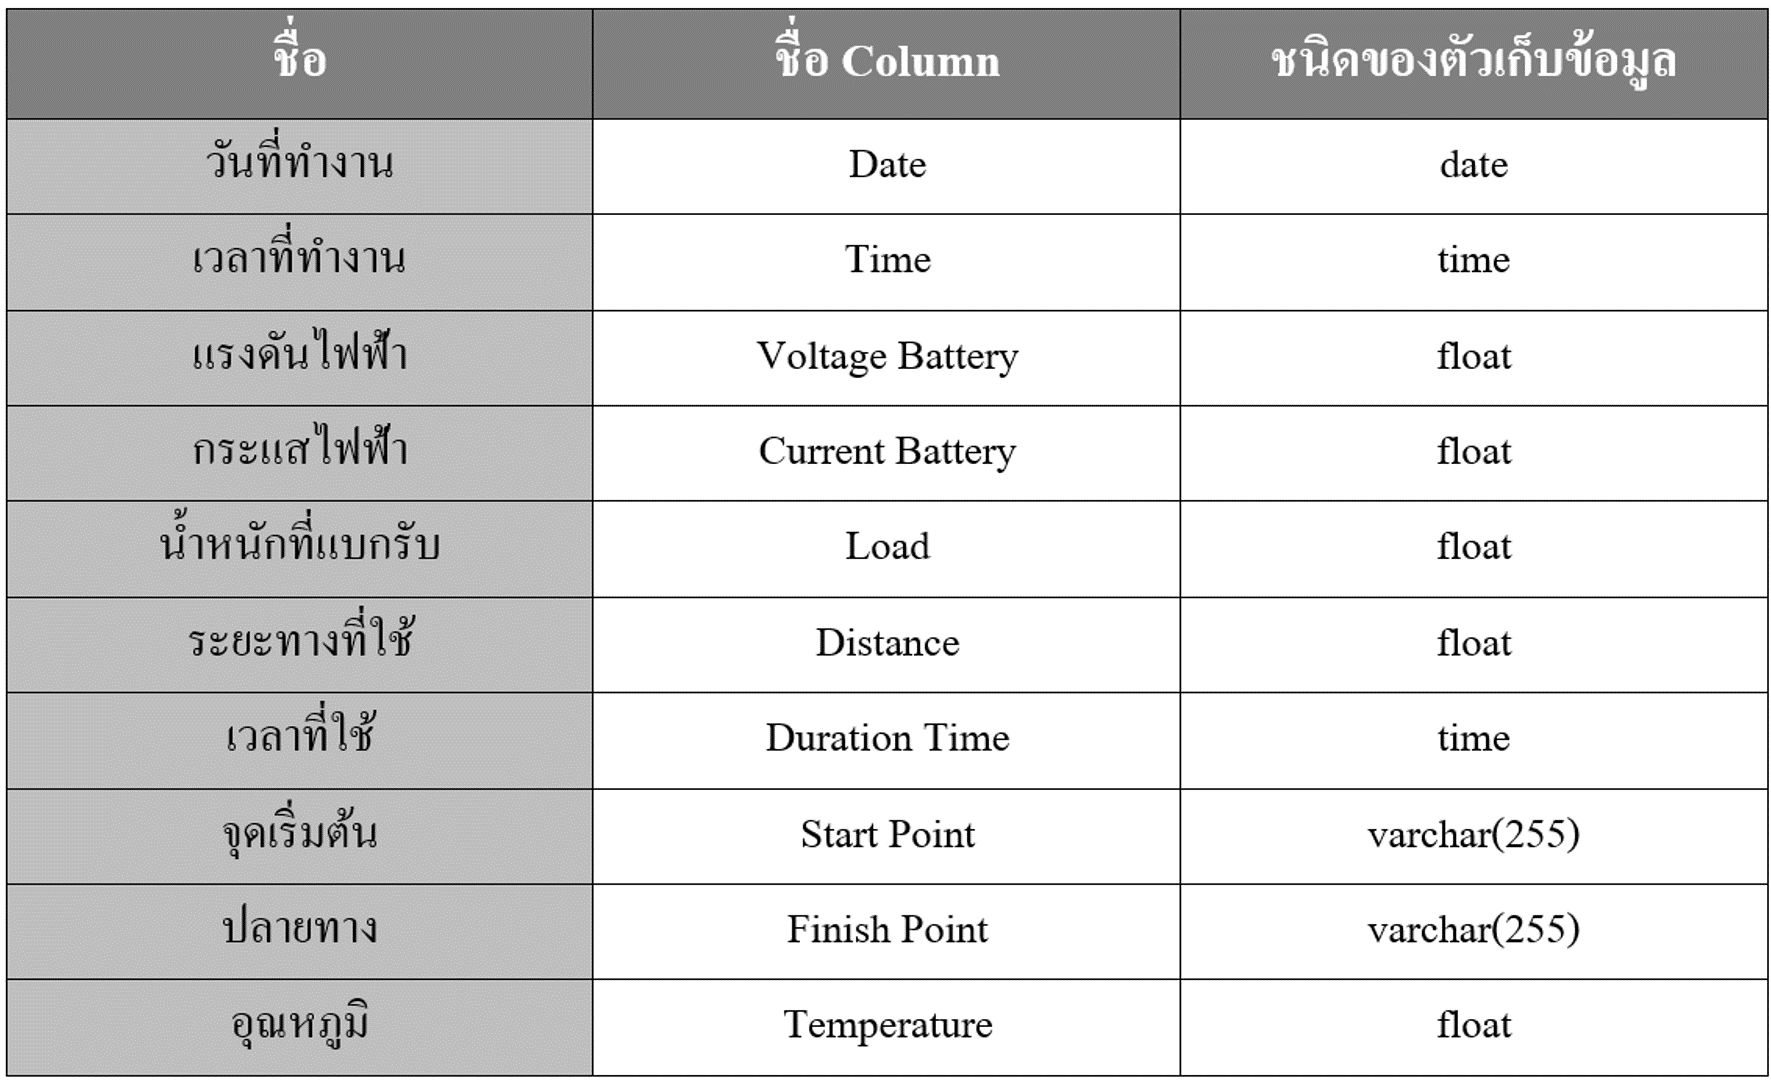
\includegraphics[width=0.9\textwidth]{images/datatype_database.png}
	\caption{ตารางแสดงชื่อและชนิดข้อมูล}
	\label{fig:datatype_database}
\end{figure}


มีการพัฒนาระบบผ่านการเขียนโปรแกรมภาษา Python บน Virtual Machine และ Query Editor
ภายใน Microsoft Azure เพื่อรับค่าที่หุ่นยนต์แต่ละตัวทำการส่งข้อมูลมาที่ Server ส่วนกลางโดยใช้รูปแบบ
MQTT จากนั้นจึงทำการอ่านค่าจากการส่งข้อมูลรูปแบบ MQTT แล้วนำไปส่งข้อมูลขึ้นไปเก็บไว้ที่ Database

\clearpage
\section{GUI for Monitor}
\begin{figure}[!ht]
	\centering
	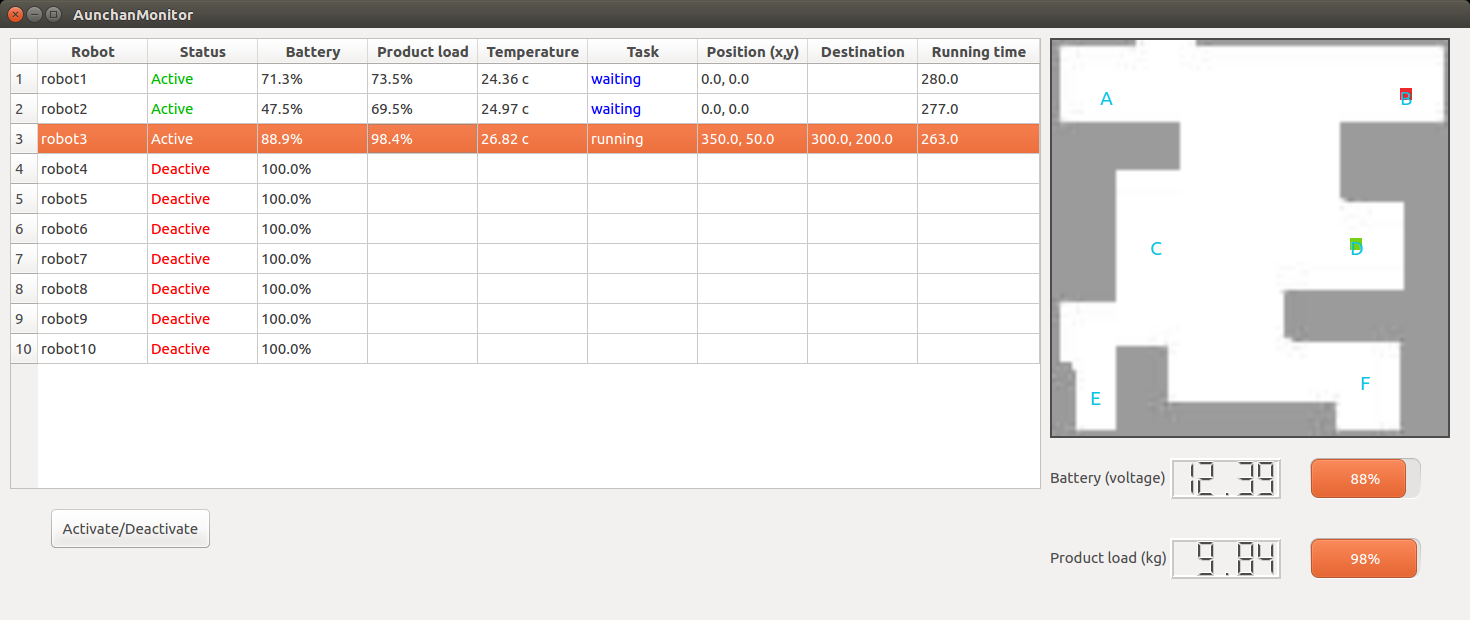
\includegraphics[width=0.9\textwidth]{images/gui_for_monitor.png}
	\caption{GUI สำหรับแสดงผลสถานะการทำงาน}
	\label{fig:gui_for_monitor}
\end{figure}

จากรูปที่ \ref{fig:gui_for_monitor} เป็นส่วนที่มีไว้เพื่อตรวจสอบสถานะต่างๆของหุ่นยนต์ ซึ่งสามารถแบ่งเป็นดังนี้
\begin{enumerate}[label=\arabic*, leftmargin=1.5cm]
	\item ชื่อ/หมายเลขของหุ่นยนต์
	\item สถานะปัจจุบัน แบ่งเป็น
	\vspace{-3mm}
	\begin{itemize}\setlength\itemsep{-0.3em}
		\item Active คือ เปิดการใช้งานอยู่
		\item Deactive คือ ไม่เปิดใช้งาน
		\item Low Battery คือ พลังงานใกล้หมด โดยคิดจากแบตเตอรี่ต่ำกว่า 15\%
		เมื่อหุ่นยนต์เข้าสู่สถานะนี้หากหุ่นยนต์มีน้ำหนักสินค้า 0\% ทำการวิ่งไปชาร์จแบตอัตโนมัติ
		แต่ถ้าหากมีน้ำหนักสินค้ามากกว่านั้นหุ่นยนต์จะทำงานต่อไป
		\item Charging คือ กำลังชาร์จพลังงาน หากหุ่นยนต์เข้าสถานะนี้จะ กลายเป็นสถานะเช่นเดียวกับ
		Deactive และ ระบบจะไปทำการ Activate หุ่นยนต์ตัวอื่น 1 ตัวอย่างอัตโนมัติ เพื่อมาทำงานแทนตนเอง 
		\item Overload คือ สินค้าที่ขนมีน้ำหนักเกิน 100\%
		\item Overheat คือ มีอุณหภูมิสูงเกินที่กำหนด 
	\end{itemize}
	\item แบตเตอร์รี่ สามารถดูได้ทั้งแบบ voltage และแบบ percent
	\item น้ำหนักของสินค้าที่อ่านได้ สามารถดูได้ทั้งแบบ kg และแบบ percent
	\item อุณหภูมิที่อ่านได้จากเซนเซอร์ มีหน่วยเป็นองศาเซลเซียส
	\item ภาระหน้าที่ แบ่งเป็น
	\vspace{-3mm}
	\begin{itemize}\setlength\itemsep{-0.3em}
		\item Waiting คือ กำลังรอเรียกใช้งานให้ไปรับ/ส่งสินค้า
		\item Running คือ ได้รับการมอบหมายงานแล้ว กำลังจะเคลื่อนที่ไปจุดที่กำหนด
	\end{itemize}
	\item ทดสอบการทำงานของหุ่นยนต์ฮิวมานอยด์
	\item ตำแหน่งของหุ่นยนต์ ณ ปัจจุบัน
	\item ตำแหน่งของจุดหมายปลายทาง
	\item เวลาการเปิดใช้งานของหุ่นยนต์ นับตั้งแต่หุ่นยนต์เปลี่ยนเป็นสถานะ Active
	\item แผนที่, ตำแหน่งของหุ่นยนต์ในแผนที่ (จุดสีแดง) และจุดหมายปลายทาง (จุดสีเขียว)
\end{enumerate}

\clearpage
\section{GUI for Control}
\begin{figure}[!ht]
	\centering
	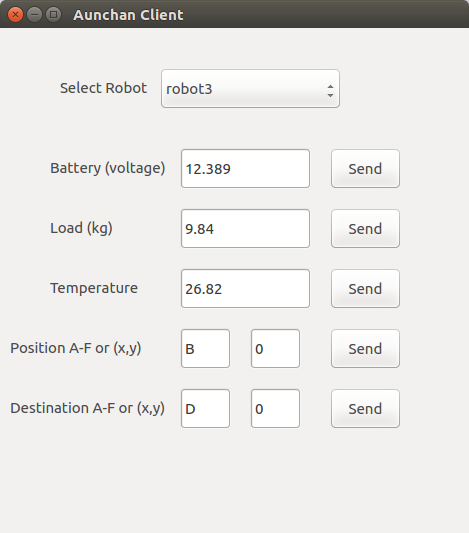
\includegraphics[width=0.5\textwidth]{images/test_gui.png}
	\caption{GUI สำหรับทดสอบการทำงาน}
	\label{fig:test_gui}
\end{figure}

จากรูปที่ \ref{fig:test_gui} มีไว้เพื่อทดลองการปรับเปลี่ยนค่าสถานะต่างๆของหุ่นยนต์ ประกอบไปด้วย
\begin{enumerate}[label=\arabic*, leftmargin=1.5cm]
	\item เลือกหุ่นยนต์ตัวที่ต้องการปรับเปลี่ยนค่า
	\item เปลี่ยนค่าแบตเตอร์โดยที่ 12.5v คือ 100\% และ 11.5v คือ 0\%
	\item เปลี่ยนค่าน้ำหนักสินค้าโดยที่ 10 kg คือ 100\% และ 0 kg คือ 0\%
	\item เปลี่ยนค่าอุณหภูมิ
	\item เปลี่ยนตำแหน่งปัจจุบันของหุ่นยนต์ โดยที่สามารถใส่ A-F เพื่อไปจุดที่ mark ไว้ในแผนที่ได้
	หรือใส่พิกัด x,y เพื่อให้ไปอยู่ตำแหน่งนั้นๆในแผนที่
	\item เปลี่ยนตำแหน่งจุดหมายปลายทางของหุ่นยนต์ โดยที่สามารถใส่ A-F เพื่อไปจุดที่ mark ไว้ในแผนที่ได้
	หรือใส่พิกัด x,y เพื่อให้ไปอยู่ตำแหน่งนั้นๆในแผนที่
\end{enumerate}

\clearpage
\section{Create map with SLAM}
\begin{figure}[!ht]
	\centering
	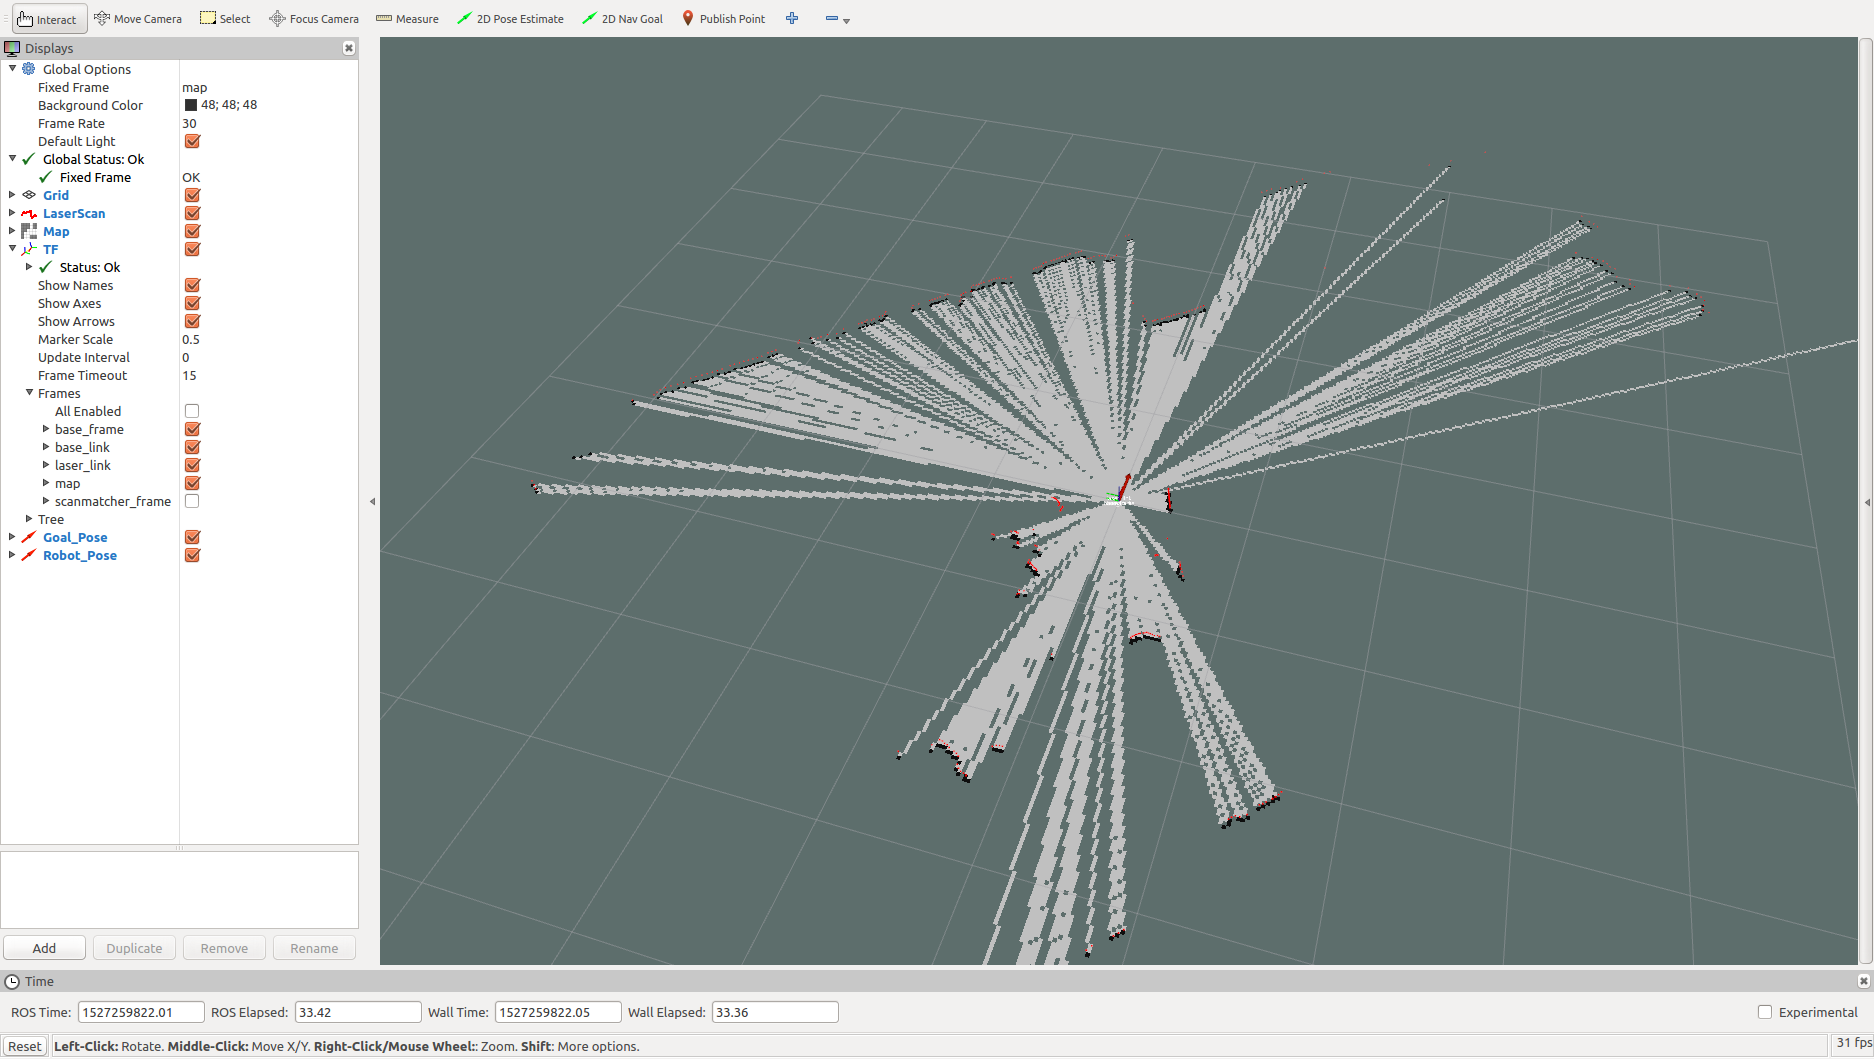
\includegraphics[width=0.9\textwidth]{images/map_slam1.png}
	\caption{ทดสอบการสร้างแผนที่ด้วย SLAM ผ่าน RViz ขั้นที่ 1}
	\label{fig:map_slam1}
\end{figure}

% \begin{figure}[!ht]
% 	\centering
% 	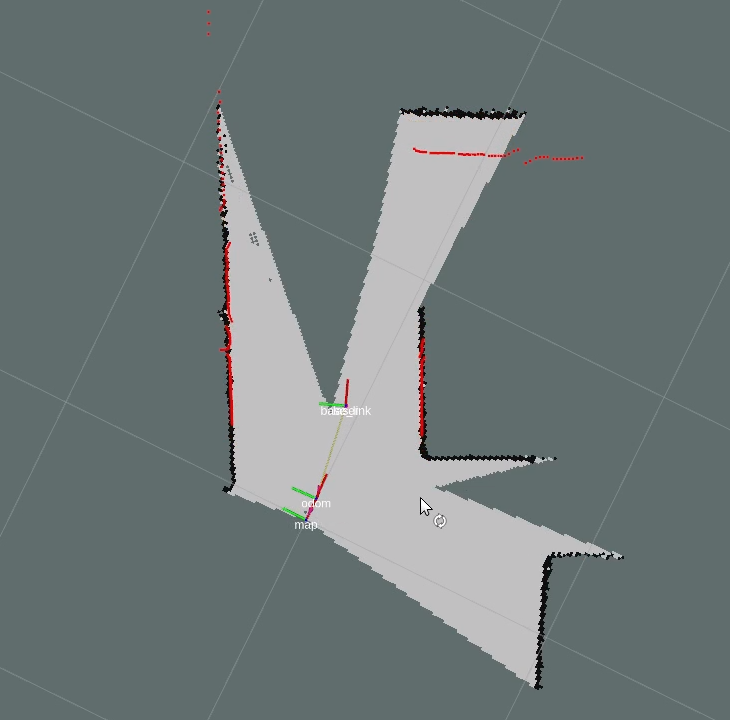
\includegraphics[width=0.7\textwidth]{images/map_slam2.png}
% 	\caption{ทดสอบการสร้างแผนที่ด้วย SLAM ผ่าน RViz ขั้นที่ 2}
% 	\label{fig:map_slam2}
% \end{figure}

\begin{figure}[!ht]
	\centering
	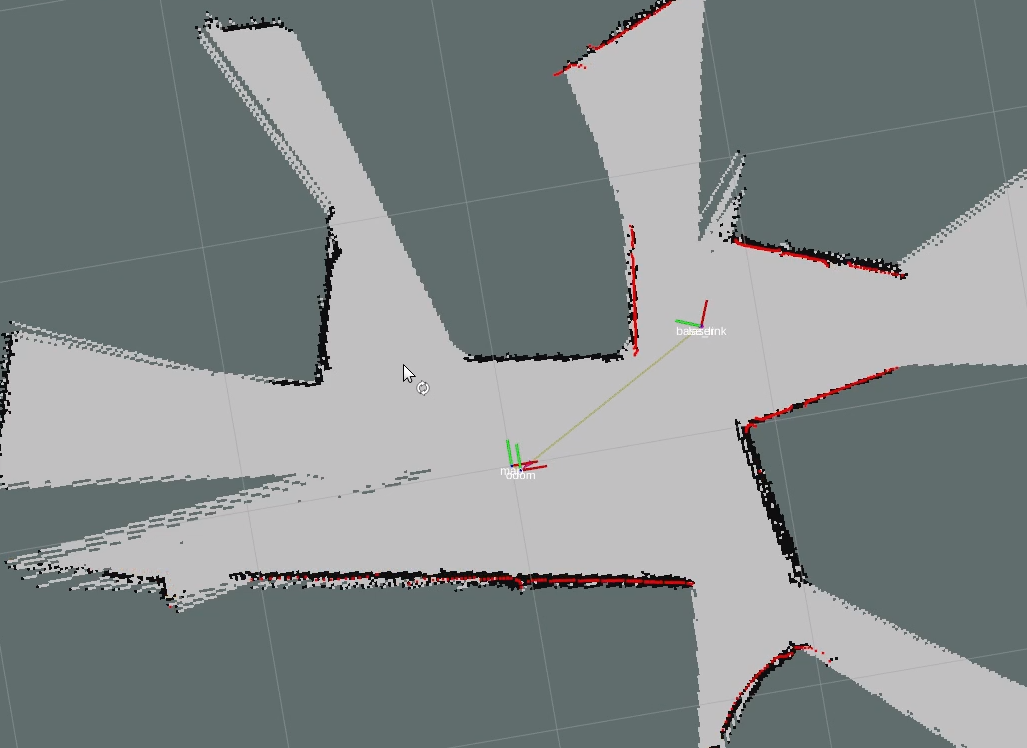
\includegraphics[width=0.9\textwidth]{images/map_slam3.png}
	\caption{ทดสอบการสร้างแผนที่ด้วย SLAM ผ่าน RViz ขั้นที่ 2}
	\label{fig:map_slam3}
\end{figure}

\clearpage
\section{Create prototype robot}
\begin{figure}[!ht]
	\centering
	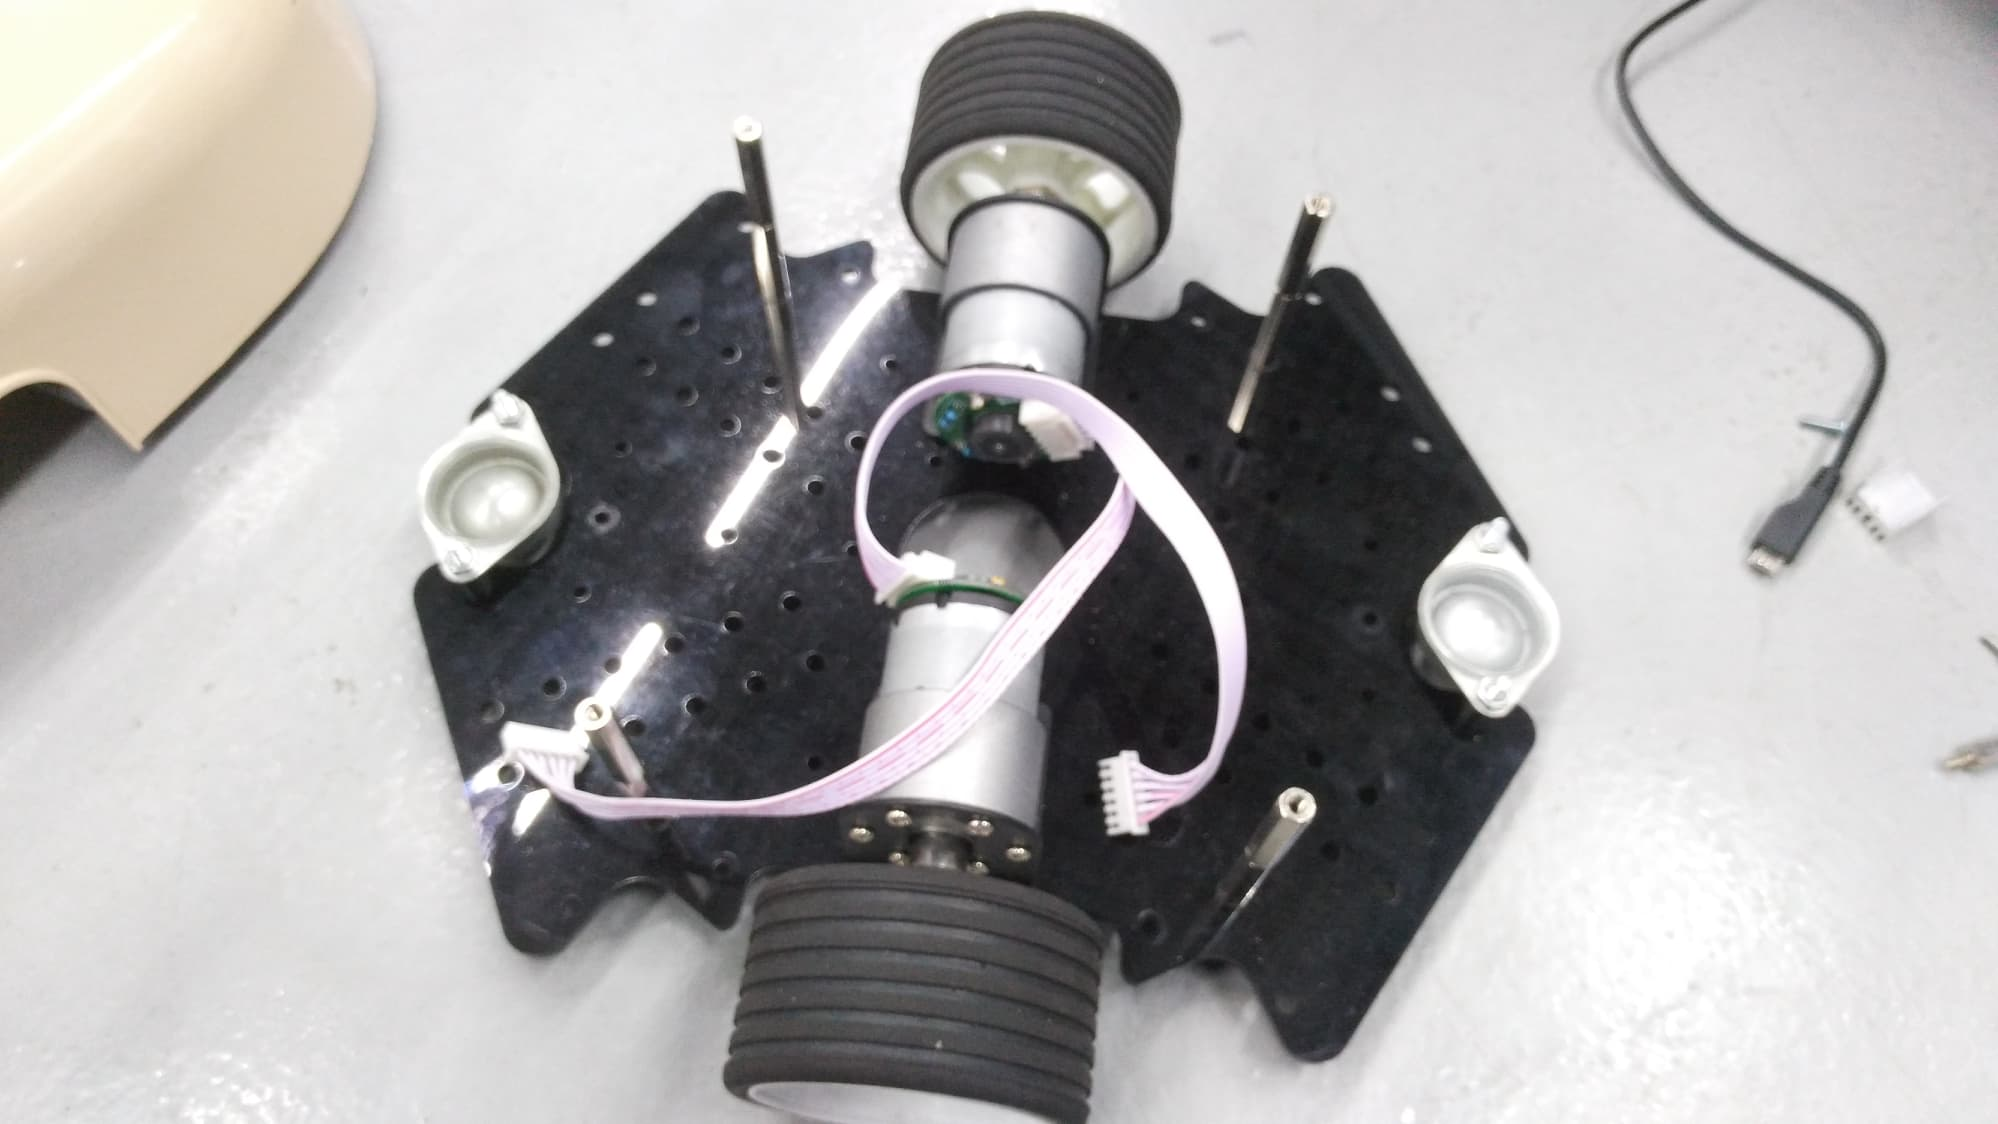
\includegraphics[width=0.7\textwidth]{images/robot_ass1.jpg}
	\caption{ขั้นตอนการประกอบหุ่นยนต์ต้นแบบ ขั้นที่ 1}
	\label{fig:robot_ass1}
\end{figure}

\begin{figure}[!ht]
	\centering
	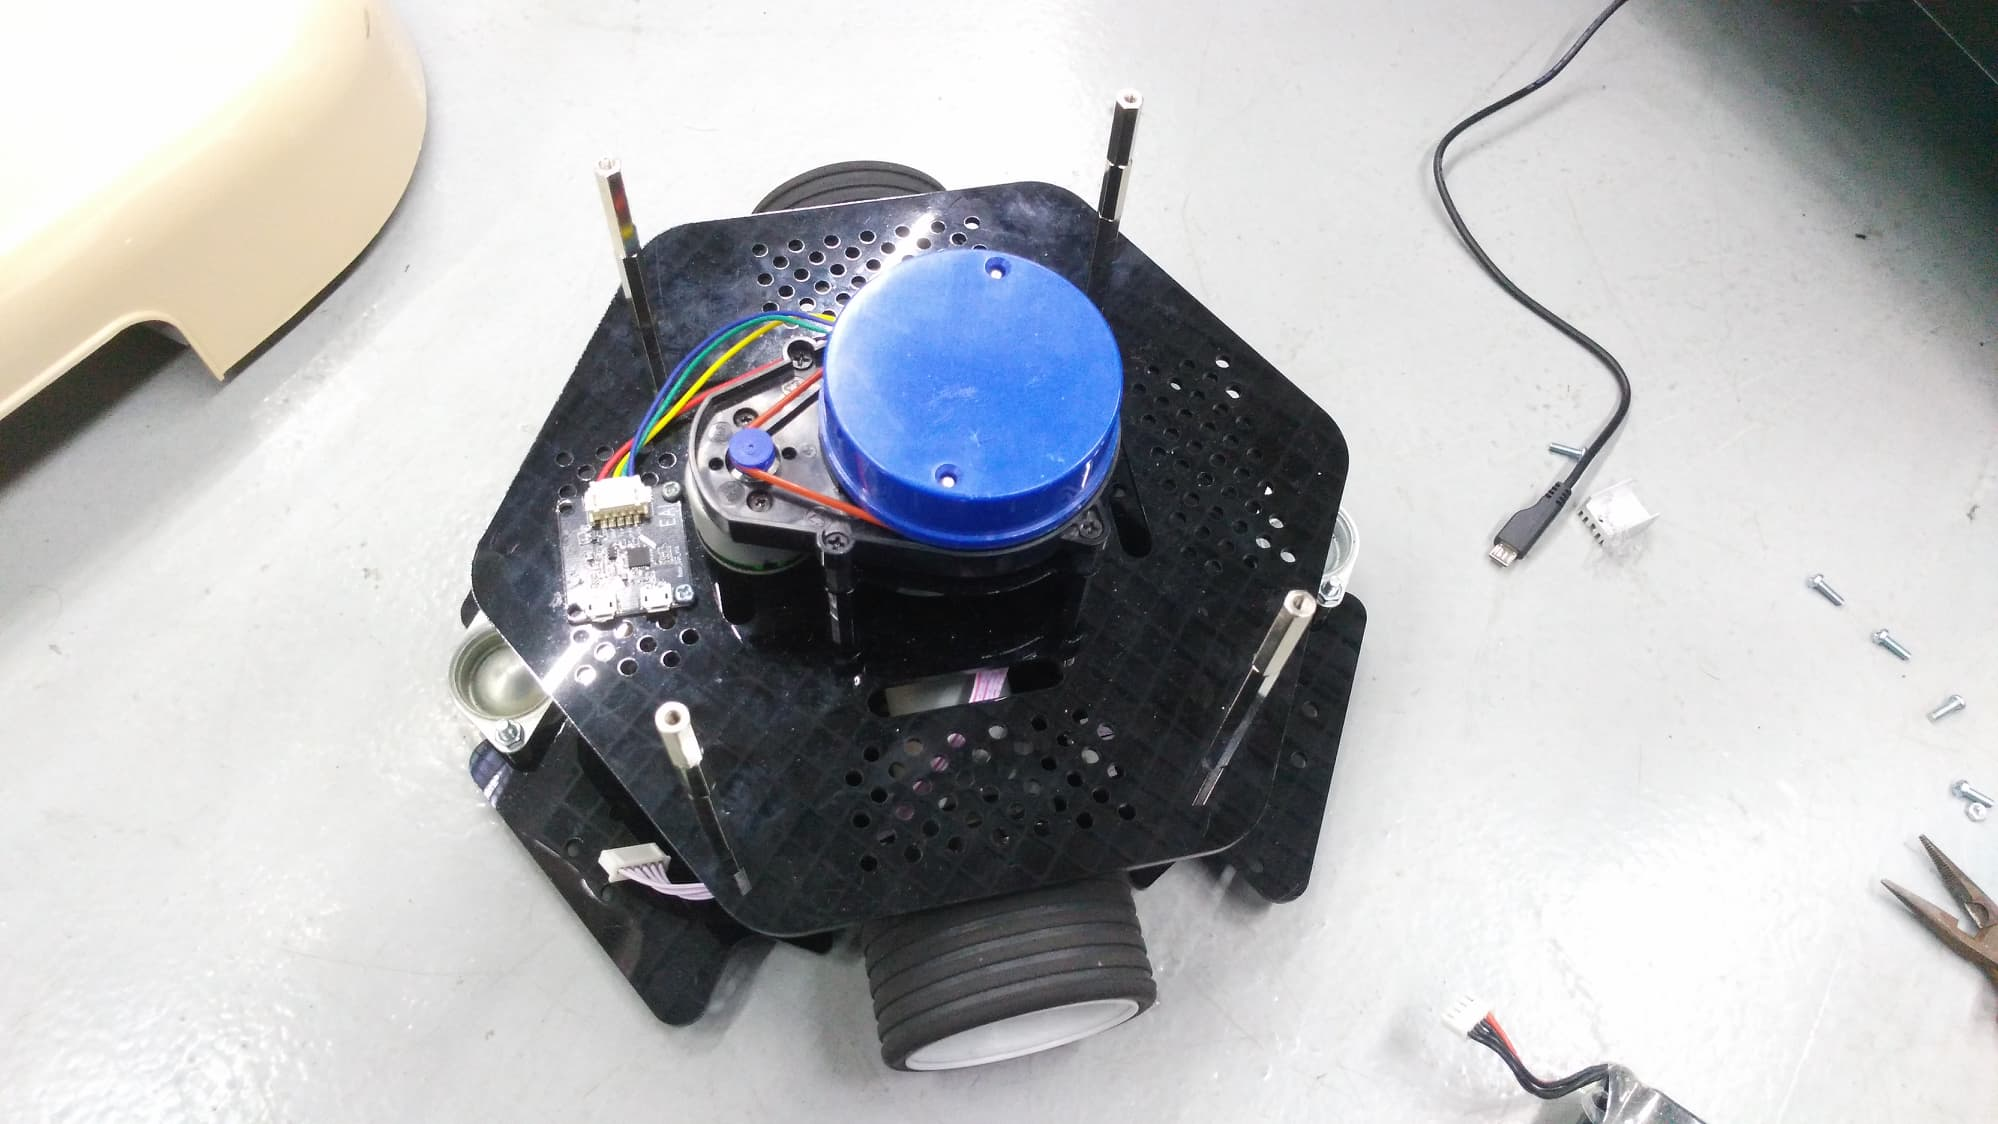
\includegraphics[width=0.7\textwidth]{images/robot_ass2.jpg}
	\caption{ขั้นตอนการประกอบหุ่นยนต์ต้นแบบ ขั้นที่ 2}
	\label{fig:robot_ass2}
\end{figure}

\begin{figure}[!ht]
	\centering
	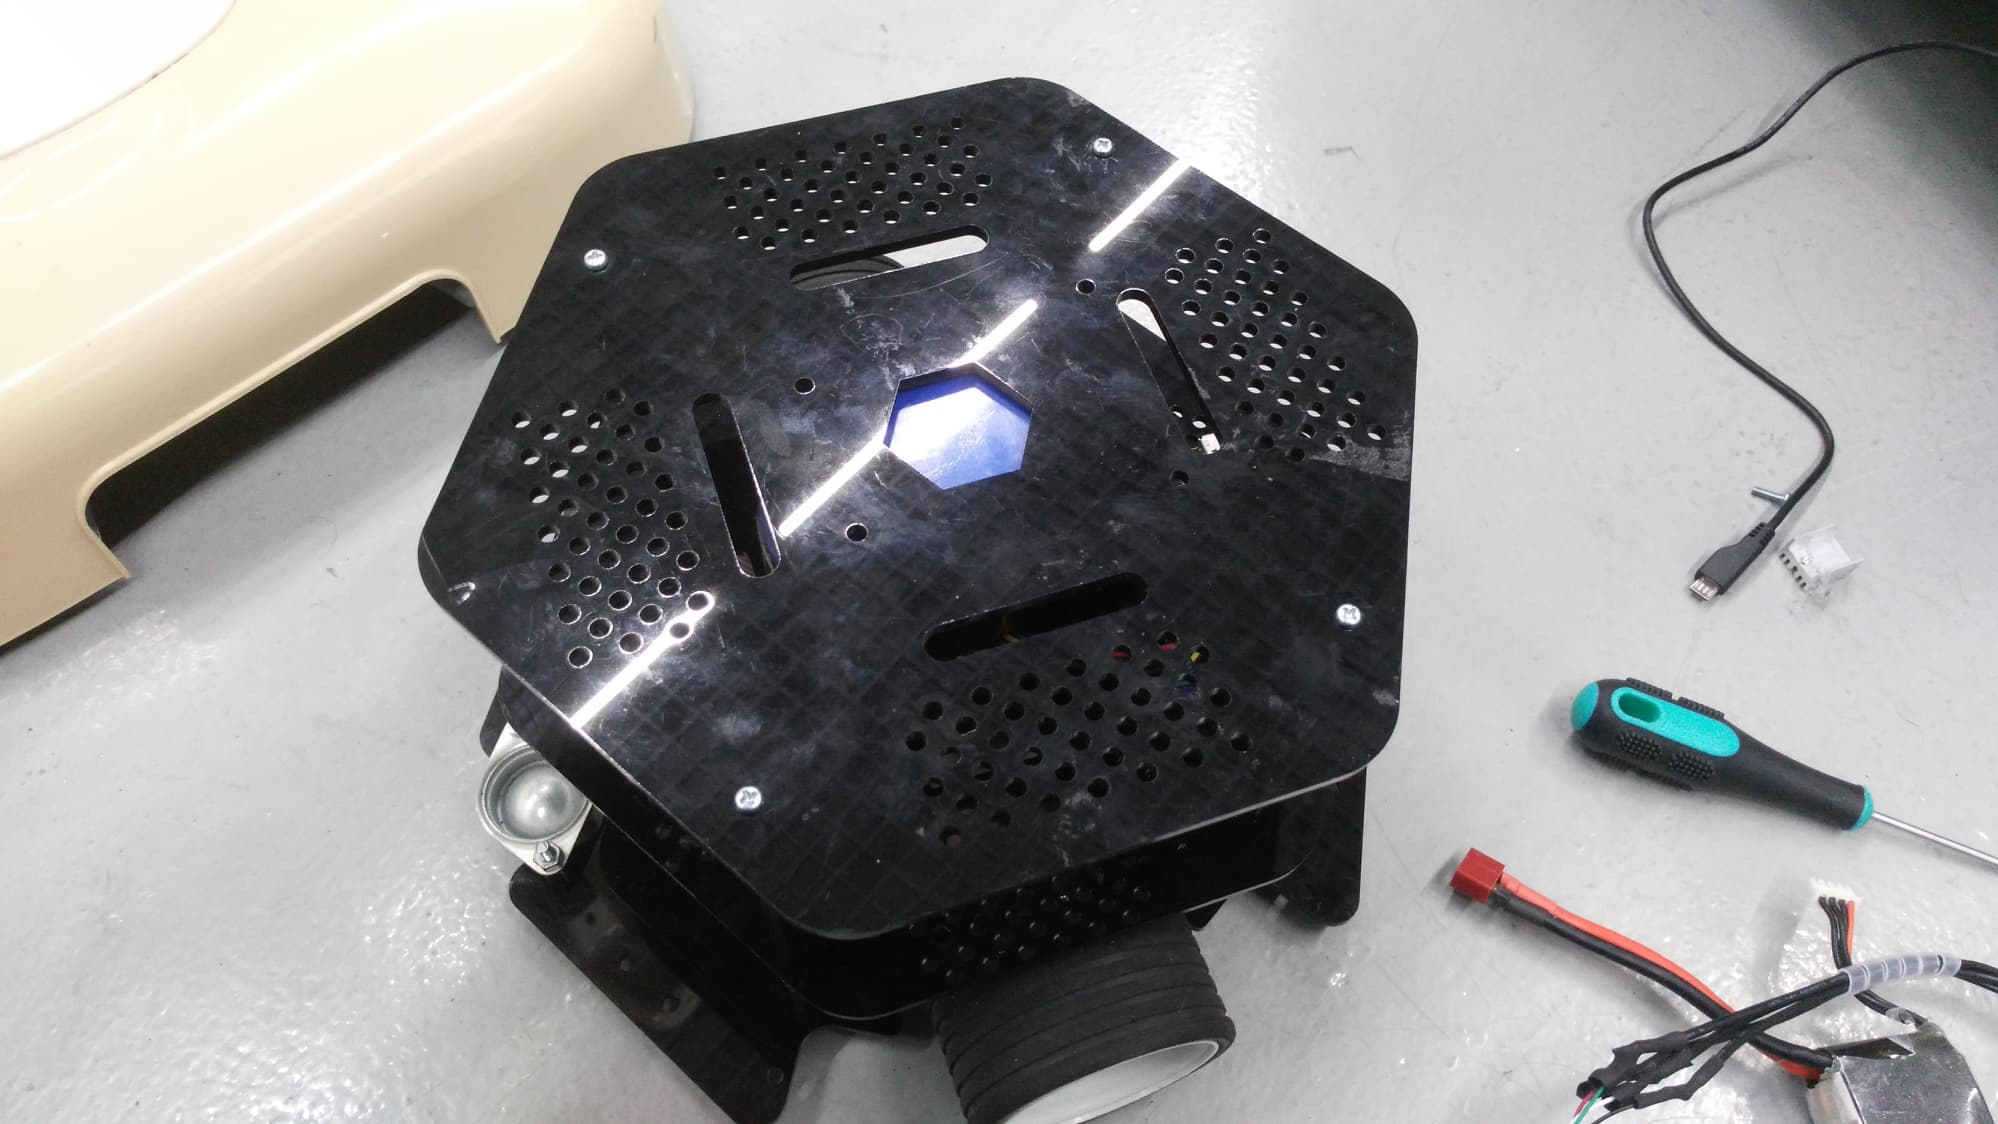
\includegraphics[width=0.7\textwidth]{images/robot_ass3.jpg}
	\caption{ขั้นตอนการประกอบหุ่นยนต์ต้นแบบ ขั้นที่ 3}
	\label{fig:robot_ass3}
\end{figure}

% \section{Quadroter mathematical model}

% \begin{figure}[htbp]
% 	\centering
% 	\includegraphics[width=0.6\textwidth]{images/Quadcopter_Coordinates.png}
% 	\caption{เฟรมอ้างอิงของโดรน}
% 	\label{fig:quadroter_coordinates}
% \end{figure}


% \chapter{Simulation}
% \chapter{...}
% \chapter{Conclusion}


\end{document}
